% Activate the following line by filling in the right side. If for example the name of the root file is Main.tex, write
% "...root = Main.tex" if the chapter file is in the same directory, and "...root = ../Main.tex" if the chapter is in a subdirectory.
 
%!TEX root =  ../Thesis.tex

\chapter[Fit Strategy and Results]{Fit Strategy and Results}

Once the data has been sent through the trigger and cuts, it is still expected
that a large number of QCD events will remain, in which there might be a (probably small)
number of signal events.  The role of the fit is to mathematically describe
the distribution of the $m_{bb}$ of all the remaining events, and to enable the
possible extraction of a signal from the background.  

This general strategy is possible because the signal events are coming from a 
resonance, the $H/A$ particle, while the background consists of a smoothly 
falling spectrum owing to the fact that it comes from various QCD processes.
That means that $H/A$, if they are present, will show up as a bump in the $m_{bb}$
spectrum.  Using the signal MC, we define what we expect for the shape of
the signal resonance (the normalization is given to us by nature, and 
is a free parameter that must be extracted if the presence of signal is identified),
while the background fit is completely data-driven.  The $m_{bb}$ ranges above
and below the signal resonance, the mass sidebands, are used to 
fit the background distribution to a polynomial, which can then be interpolated
into the signal region.  That allows us to test the goodness-of-fit for a 
background-only hypothesis against the fit quality for a signal+background
hypothesis, for various signal normalizations.  These fit results are then
the ingredients for the limit-setting procedure, which is detailed in the next section.

This chapter details the various categories that are used in the fit, and
the parametric forms that are used to fit them.   

\subsection{Fit Model and Categories}
\label{subsec:fitmodel}
The fit is performed in several different categories, which vary in the 
signal/background ratio, the signal and background shapes, and the
absolute normalizations of the signal and background.  In a situation like
this, where there are several categories that can be defined and the
search sensitivity varies depending on which category is being examined,
it can benefit the overall search sensitivity to fit each category 
separately and then combine them at the end.  While the parameteric form
of the fit is the same in each category (background fit with a polynomial, 
signal fit with a type of bifurcated Gaussian), the categories are fit
separately and so the exact values of the parameters found by the fit
will be slightly different.  


The statistical analysis of the data employs an unbinned likelihood
function, defined as:
\begin{equation}
\text{Pois}(N|\mu S+B) \prod_{k=1}^{njet\ cat} \prod_{l=1}^{N_{tag\ cat}} \prod_{i=1}^{N_{l}} \left[ \mu N_{S,k,l} PDF_{sig,k,l}(m_{bb,i}) + N_{B,k,l} PDF_{bkg}(m_{bb,i}) \right]
\end{equation}
where:
\begin{itemize}
\item the product is over the $b$-tag categories $l$, the n$_{jets}$ categores $k$, and over the events in each category $i$;
\item $N_{S,l}$ and $N_{B,l}$ are the expected signal and background yield in each category;
\item $PDF_{sig,l}(m_{bb})$ and $PDF_{bkg}(m_{bb})$ are the signal and background probability density functions for  the different categories;
\item $\mu$ is a signal strength which multiplies the overall signal prediction.
\end{itemize}


The $b$-tag fit categories $l$ are three exclusive categories to which events are assigned
based on the $b$-tag value of the third-most $b$-jet-like jet in the event (the two most
$b$-like jets have already been $b$-tagged in the trigger, and are assumed to be true
$b$-jets).  Then the categorization in $b$-tag fit categories splits the sample into three
regions with different signal and background enrichments:


\begin{itemize}
    \item $bbb$: one or more jets (in addition to the two triple-tagged jets) passing a tight (60\% working point)
 MV1 cut–-in effect, the full signal selection criteria
    \item $bbloose$: events failing the bbb classification but which have one or more jets passing a loose (80\%
working point) MV1 cut
    \item $bbanti$: events that have no jets passing an 80\% MV1 cut-–effectively a veto on the presence of any
b-tagged jets other than those firing the trigger
\end{itemize}

When assigning events to one of these categories, we only allow $b$-tags on the leading
five jets to count toward the $bbb$ or $bbloose$ categories.  In other words, if the third
$b$-tagged jet in an event is the 6th jet (in $p_T$ ordering) overall, the event 
will be classified as $bbanti$.  This requirement is motivated by our physics awareness that
the $b$-jets coming from signal events should be fairly high $p_T$, so this should have
a minimal effect of rejecting signal that would otherwise be accepted.  On the other
hand, with high-jet-multiplicity QCD events, there is the combinatorial effect of looking across
more jets for $b$-tags that increases the likelihood of an event being classified as signal-like
(bbb or bbloose) as there are more jets in the event.  Only looking at the leading 5 jets
for $b$-tags keeps this effect under control. 


The second type of categorization is based on the number of 
jets in the event: 3, 4, or 5 or more jets.  We find that the signal
shape can change based on the number of events, as well as the overall
signal and background normalizations.  For more details on the effect of 
the number of jets on the signal distributions, see Section~\ref{sec:n_jets_sig}. 




\subsection{PDF Shapes and Fit Constraints}
\label{sec:pdfs}

\subsubsection{Exponential-Only Fit to Background}
The background distribution is generally well-described by a decaying exponential, 
as long as the fit window begins past the turn-on region.  An exponential has the
additional advantages of only having one degree of freedom (the decay constant), 
making convergence relatively straightforward, as well as a mathematical guarantee
to be monotonically decreasing, obviating the concern that wiggles in the background
shape could absorb a possible signal.






\subsubsection{Exponential Plus Logistic Fit to Background}
While an exponential distribution does an admirable job of describing the bulk of the
distribution, an examination of the residual errors shows that it systematically 
overshoots the low end of the $m_{bb}$ distribution, and undershoots
the high end.  These errors look like they might be well-described by a logistic
function, so this as added as a correction in the 4-jet and 5-jet bins (the 3-jet
bin does not seem to suffer from this bias).  




\subsubsection{Cruijff Fit to Signal}

%http://www.slac.stanford.edu/econf/C0303241/proc/pres/502.PDF
The signal $m_{bb}$ shape is fit with a Cruijff PDF.  The Cruijff function is a bifurcated Gaussian (different widths for left and right sides of the distribution) with non-Gaussian tails: 

\begin{equation}
f(x) = exp((x-m_{bb})^2 / (2\sigma^2_{L,R} + \alpha_{L,R}(x-m)^2))
\end{equation}

The signal MC distributions and fit results can be seen in Figures
~\ref{fig:signalPDFs_3j}-~\ref{fig:signalPDFs_5j_bbloose}. 


\begin{figure}[phtb!]
  \begin{center}
  \begin{subfigure}[$m_{A}=400$ GeV]{0.4\textwidth}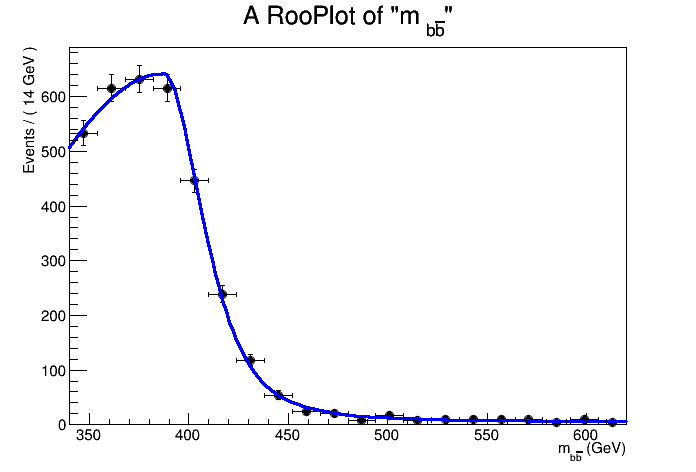
\includegraphics[width=\textwidth]{FitResults/images/fitMC_bAbb400_1.png}\end{subfigure}
  \begin{subfigure}[$m_{A}=450$ GeV]{0.4\textwidth}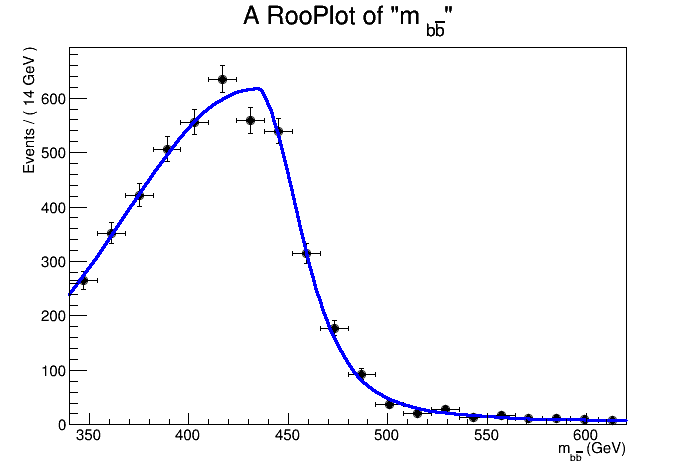
\includegraphics[width=\textwidth]{FitResults/images/fitMC_bAbb450_1.png}\end{subfigure}
  \begin{subfigure}[$m_{A}=500$ GeV]{0.4\textwidth}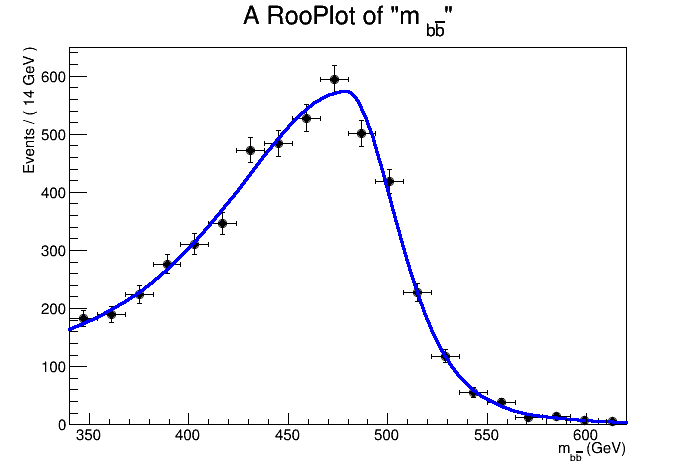
\includegraphics[width=\textwidth]{FitResults/images/fitMC_bAbb500_1.png}\end{subfigure}
  \begin{subfigure}[$m_{A}=550$ GeV]{0.4\textwidth}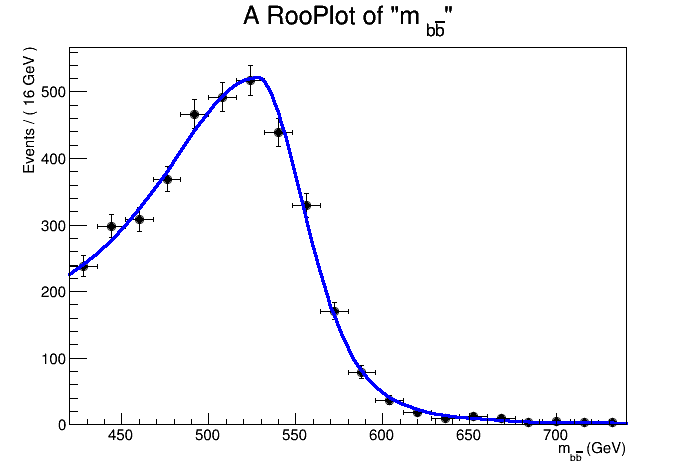
\includegraphics[width=\textwidth]{FitResults/images/fitMC_bAbb550_1.png}\end{subfigure}
  \begin{subfigure}[$m_{A}=600$ GeV]{0.4\textwidth}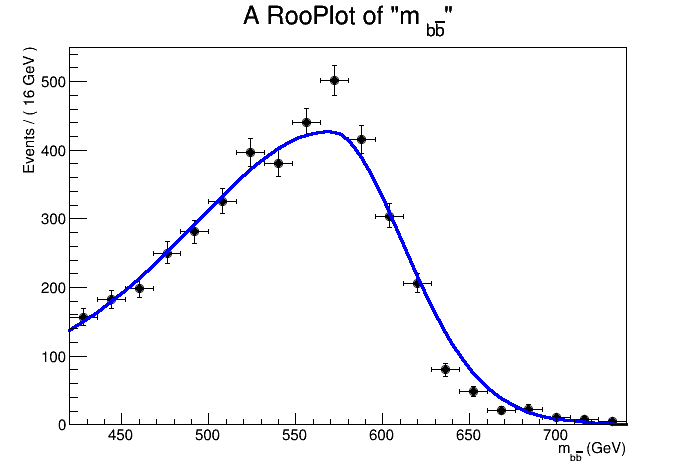
\includegraphics[width=\textwidth]{FitResults/images/fitMC_bAbb600_1.png}\end{subfigure}
  \begin{subfigure}[$m_{A}=650$ GeV]{0.4\textwidth}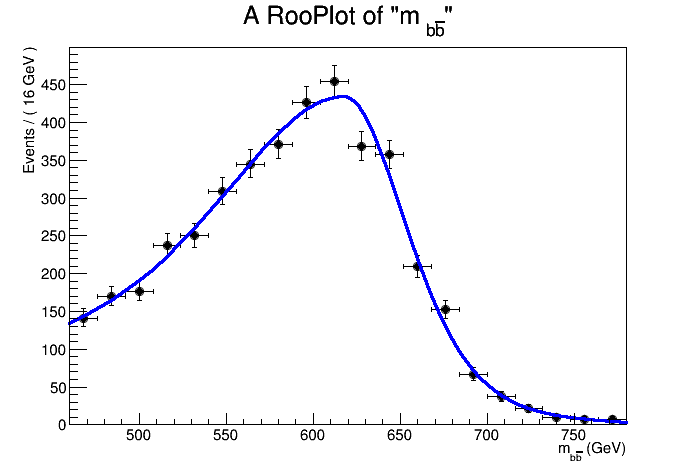
\includegraphics[width=\textwidth]{FitResults/images/fitMC_bAbb650_1.png}\end{subfigure}
  \begin{subfigure}[$m_{A}=700$ GeV]{0.4\textwidth}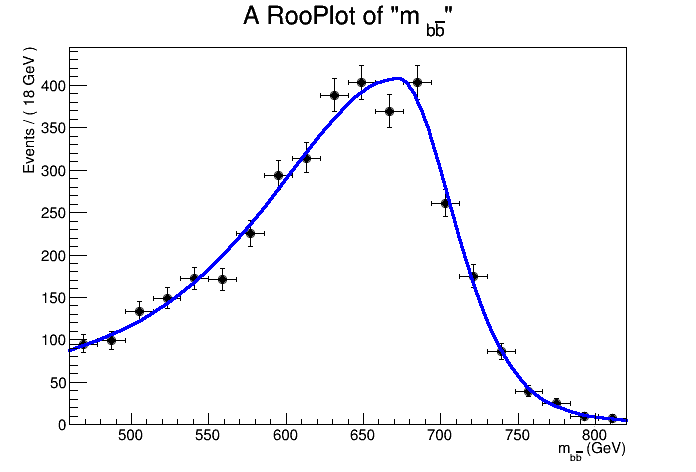
\includegraphics[width=\textwidth]{FitResults/images/fitMC_bAbb700_1.png}\end{subfigure}
  \begin{subfigure}[$m_{A}=800$ GeV]{0.4\textwidth}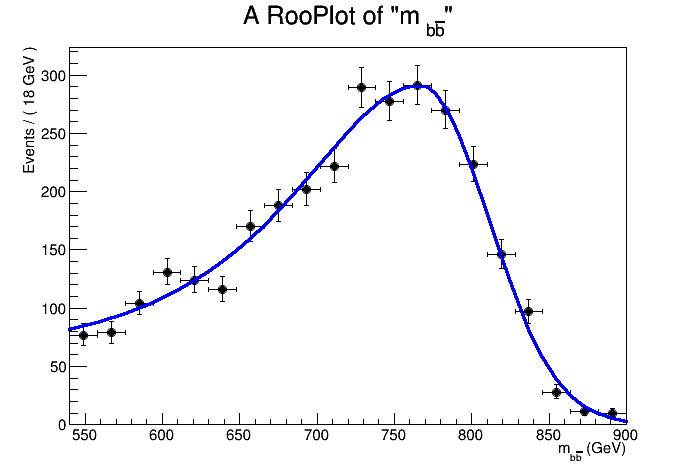
\includegraphics[width=\textwidth]{FitResults/images/fitMC_bAbb800_1.png}\end{subfigure}
  \caption{Signal MC distributions and Cruijff PDFs for $m_{bb}$ in the {\it bbb} category, for events with 3 jets, for different $H/A$ masses. \label{fig:signalPDFs_3j}}
    \end{center}
\end{figure}


\begin{figure}[phtb!]
  \begin{center}
  \begin{subfigure}[$m_{A}=400$ GeV]{0.4\textwidth}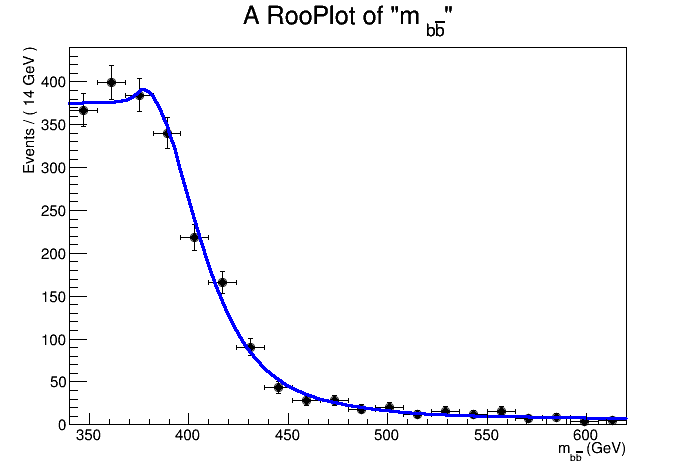
\includegraphics[width=\textwidth]{FitResults/images/fitMC_bAbb400_2.png}\end{subfigure}
  \begin{subfigure}[$m_{A}=450$ GeV]{0.4\textwidth}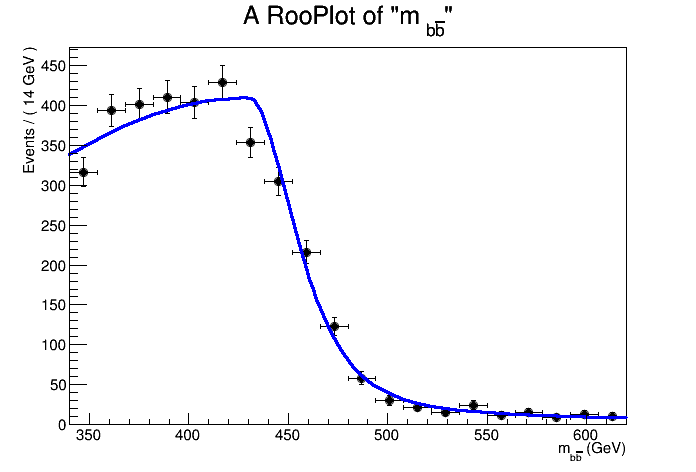
\includegraphics[width=\textwidth]{FitResults/images/fitMC_bAbb450_2.png}\end{subfigure}
  \begin{subfigure}[$m_{A}=500$ GeV]{0.4\textwidth}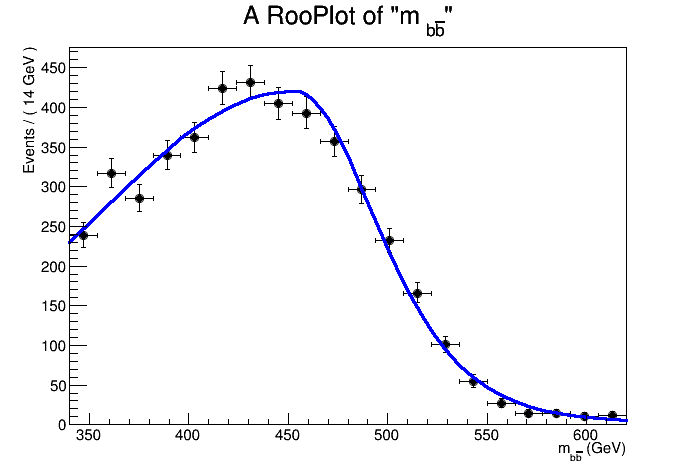
\includegraphics[width=\textwidth]{FitResults/images/fitMC_bAbb500_2.png}\end{subfigure}
  \begin{subfigure}[$m_{A}=550$ GeV]{0.4\textwidth}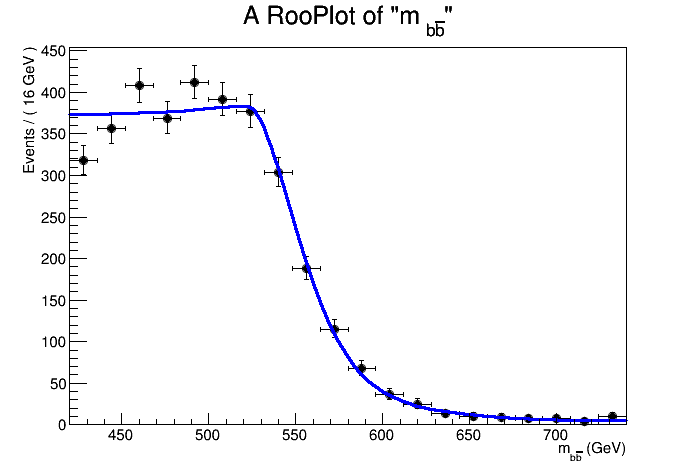
\includegraphics[width=\textwidth]{FitResults/images/fitMC_bAbb550_2.png}\end{subfigure}
  \begin{subfigure}[$m_{A}=600$ GeV]{0.4\textwidth}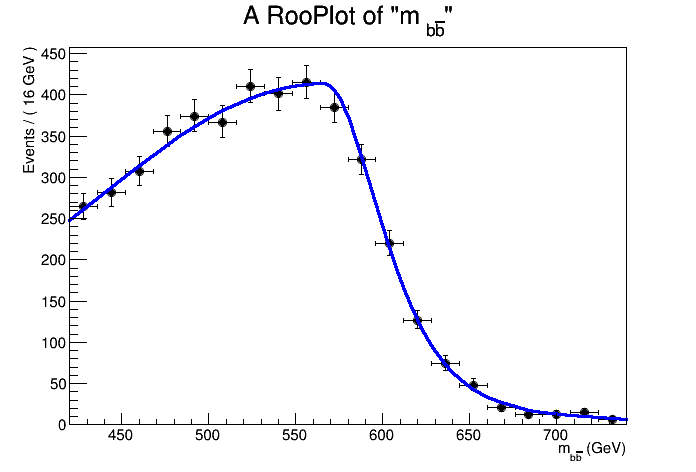
\includegraphics[width=\textwidth]{FitResults/images/fitMC_bAbb600_2.png}\end{subfigure}
  \begin{subfigure}[$m_{A}=650$ GeV]{0.4\textwidth}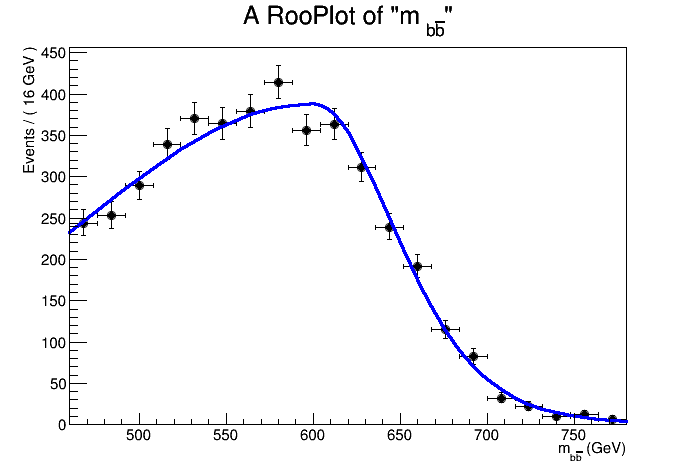
\includegraphics[width=\textwidth]{FitResults/images/fitMC_bAbb650_2.png}\end{subfigure}
  \begin{subfigure}[$m_{A}=700$ GeV]{0.4\textwidth}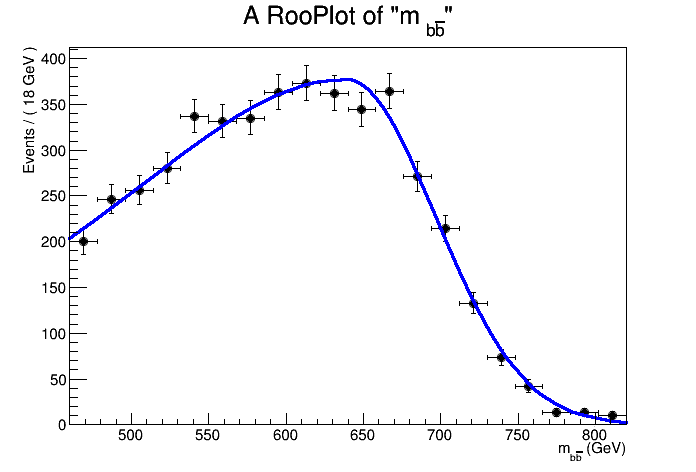
\includegraphics[width=\textwidth]{FitResults/images/fitMC_bAbb700_2.png}\end{subfigure}
  \begin{subfigure}[$m_{A}=800$ GeV]{0.4\textwidth}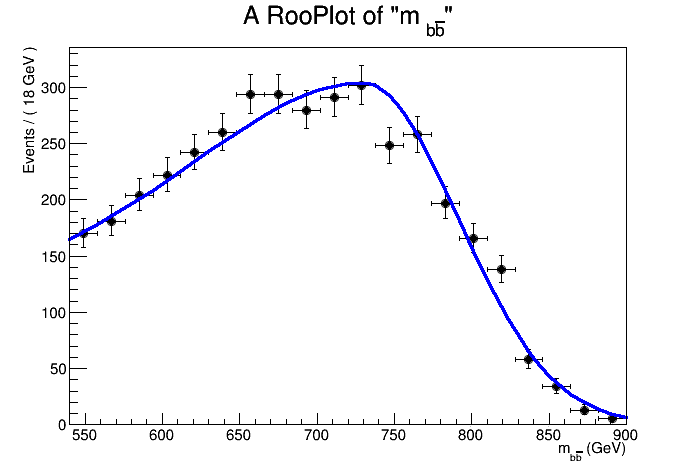
\includegraphics[width=\textwidth]{FitResults/images/fitMC_bAbb800_2.png}\end{subfigure}
  \caption{Signal MC distributions and Cruijff PDFs for $m_{bb}$ in the {\it bbb} category, for events with 4 jets, for different $H/A$ masses. \label{fig:signalPDFs_4j}}
    \end{center}
\end{figure}

\begin{figure}[phtb!]
  \begin{center}
  \begin{subfigure}[$m_{A}=400$ GeV]{0.4\textwidth}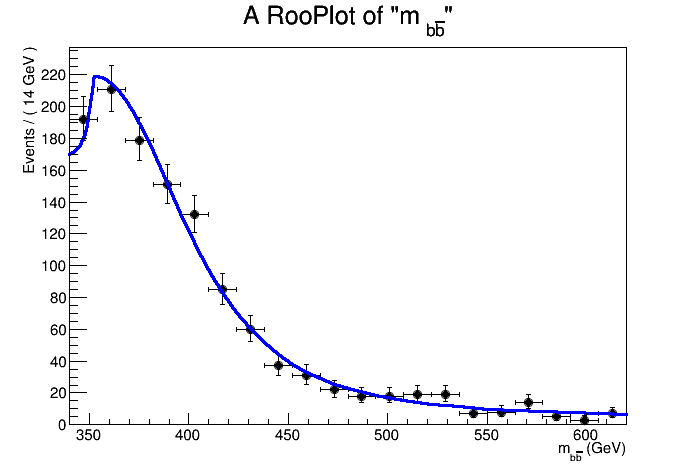
\includegraphics[width=\textwidth]{FitResults/images/fitMC_bAbb400_3.png}\end{subfigure}
  \begin{subfigure}[$m_{A}=450$ GeV]{0.4\textwidth}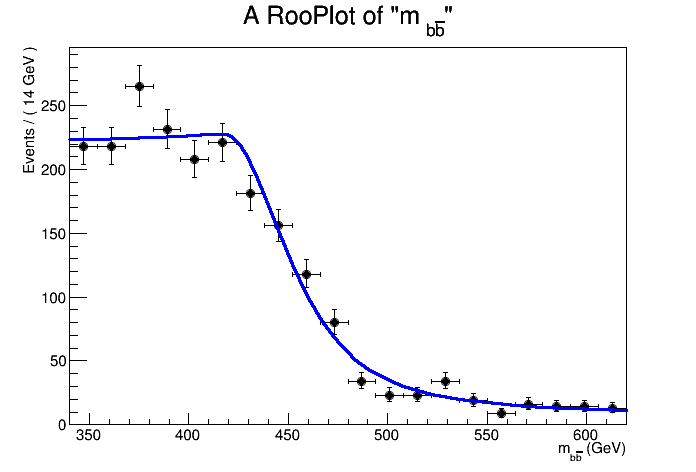
\includegraphics[width=\textwidth]{FitResults/images/fitMC_bAbb450_3.png}\end{subfigure}
  \begin{subfigure}[$m_{A}=500$ GeV]{0.4\textwidth}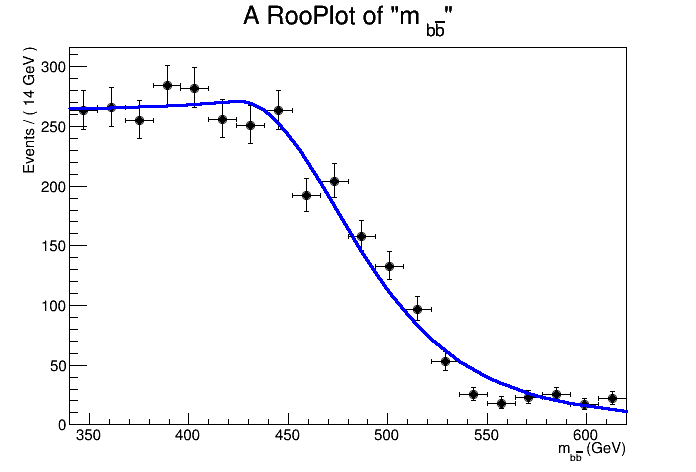
\includegraphics[width=\textwidth]{FitResults/images/fitMC_bAbb500_3.png}\end{subfigure}
  \begin{subfigure}[$m_{A}=550$ GeV]{0.4\textwidth}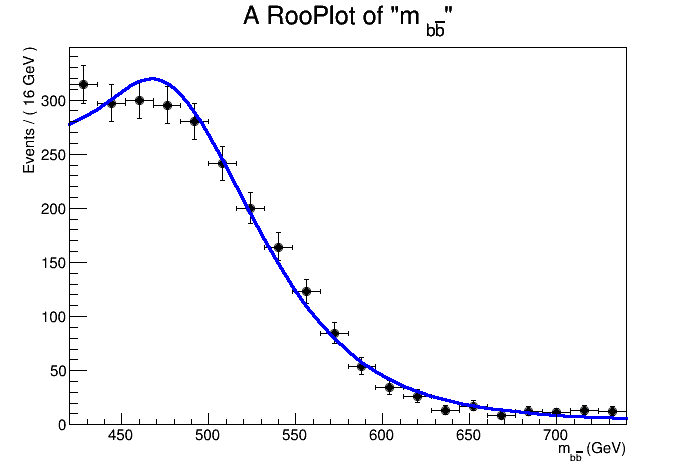
\includegraphics[width=\textwidth]{FitResults/images/fitMC_bAbb550_3.png}\end{subfigure}
  \begin{subfigure}[$m_{A}=600$ GeV]{0.4\textwidth}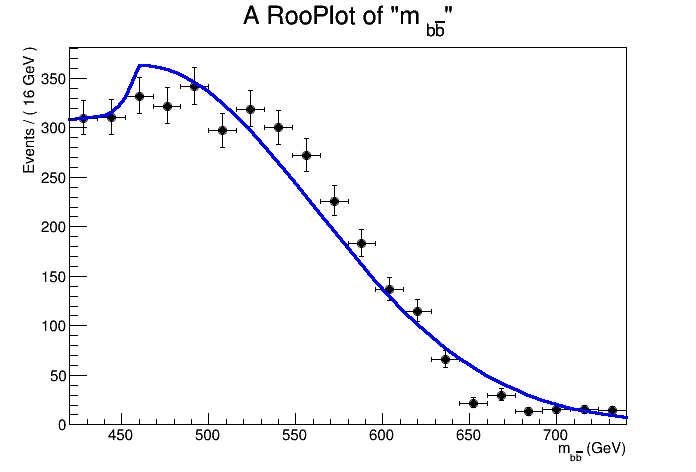
\includegraphics[width=\textwidth]{FitResults/images/fitMC_bAbb600_3.png}\end{subfigure}
  \begin{subfigure}[$m_{A}=650$ GeV]{0.4\textwidth}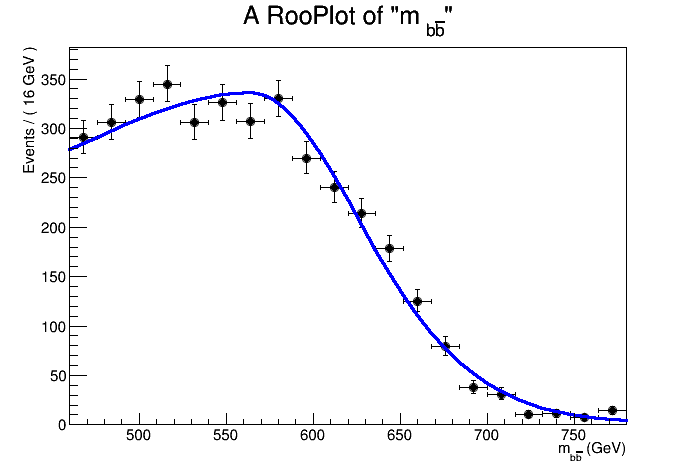
\includegraphics[width=\textwidth]{FitResults/images/fitMC_bAbb650_3.png}\end{subfigure}
  \begin{subfigure}[$m_{A}=700$ GeV]{0.4\textwidth}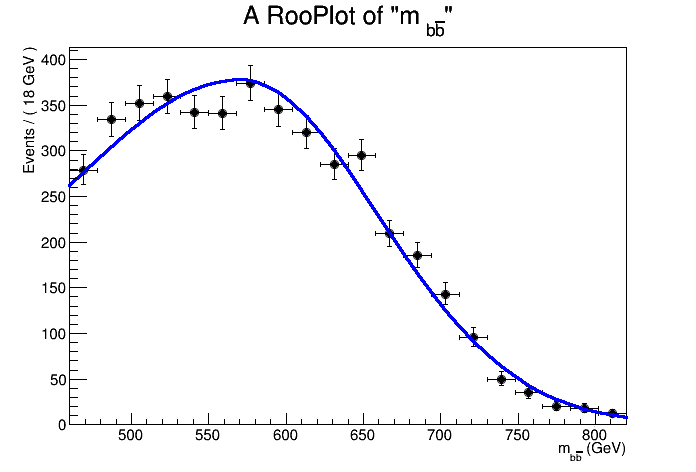
\includegraphics[width=\textwidth]{FitResults/images/fitMC_bAbb700_3.png}\end{subfigure}
  \begin{subfigure}[$m_{A}=800$ GeV]{0.4\textwidth}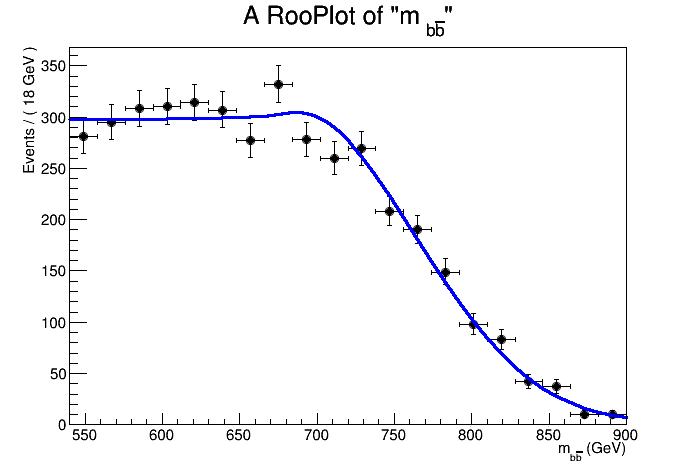
\includegraphics[width=\textwidth]{FitResults/images/fitMC_bAbb800_3.png}\end{subfigure}
  \caption{Signal MC distributions and Cruijff PDFs for $m_{bb}$ in the {\it bbb} category, for events with 5 or more jets, for different $H/A$ masses. \label{fig:signalPDFs_5j}}
    \end{center}
\end{figure}







\begin{figure}[phtb!]
  \begin{center}
  \begin{subfigure}[$m_{A}=400$ GeV]{0.4\textwidth}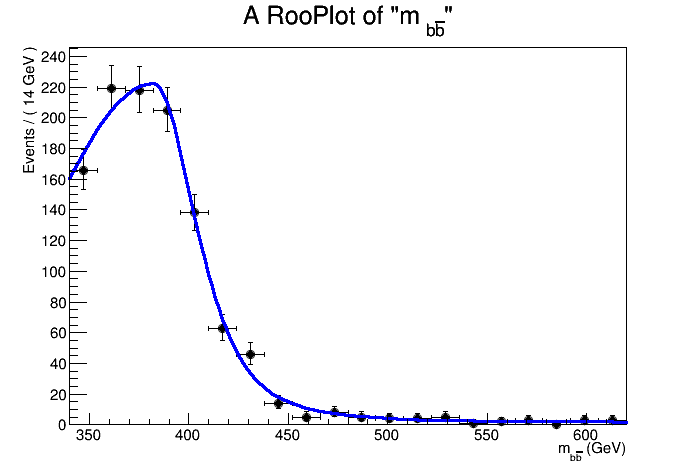
\includegraphics[width=\textwidth]{FitResults/images/fitMC_bAbb400_4.png}\end{subfigure}
  \begin{subfigure}[$m_{A}=450$ GeV]{0.4\textwidth}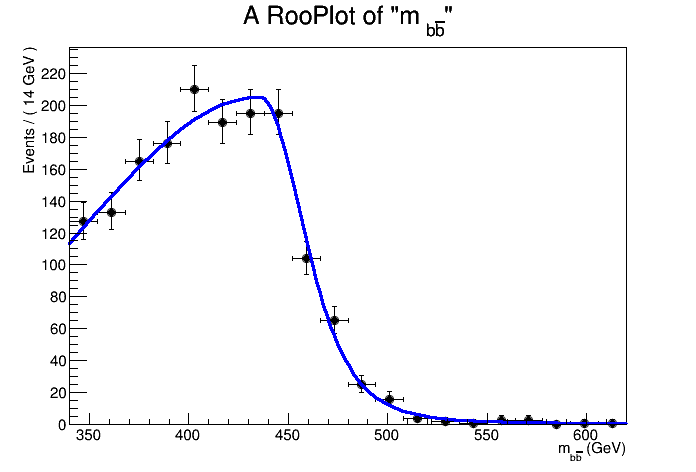
\includegraphics[width=\textwidth]{FitResults/images/fitMC_bAbb450_4.png}\end{subfigure}
  \begin{subfigure}[$m_{A}=500$ GeV]{0.4\textwidth}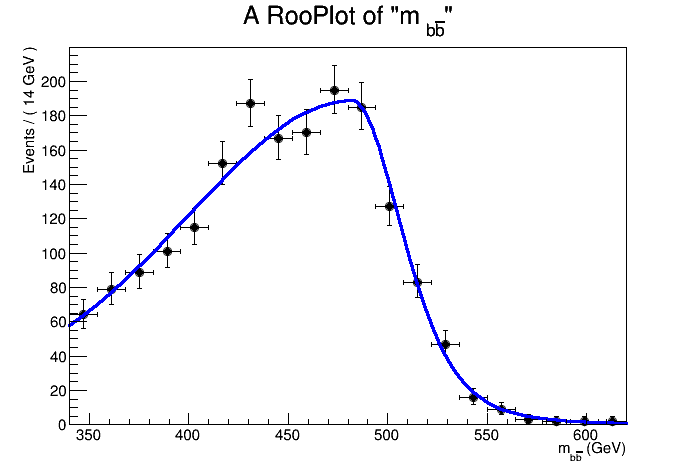
\includegraphics[width=\textwidth]{FitResults/images/fitMC_bAbb500_4.png}\end{subfigure}
  \begin{subfigure}[$m_{A}=550$ GeV]{0.4\textwidth}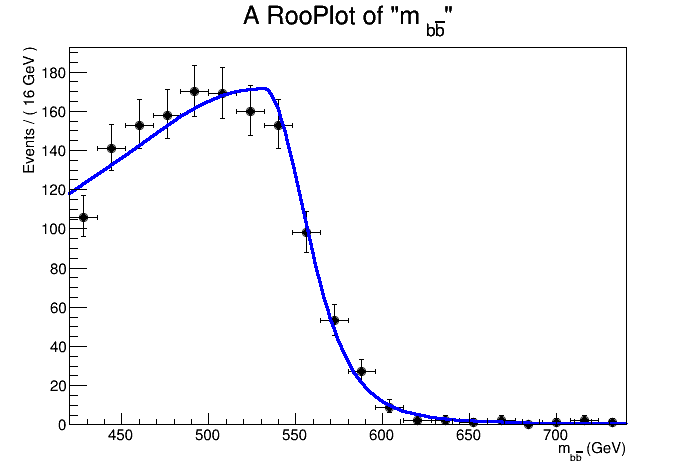
\includegraphics[width=\textwidth]{FitResults/images/fitMC_bAbb550_4.png}\end{subfigure}
  \begin{subfigure}[$m_{A}=600$ GeV]{0.4\textwidth}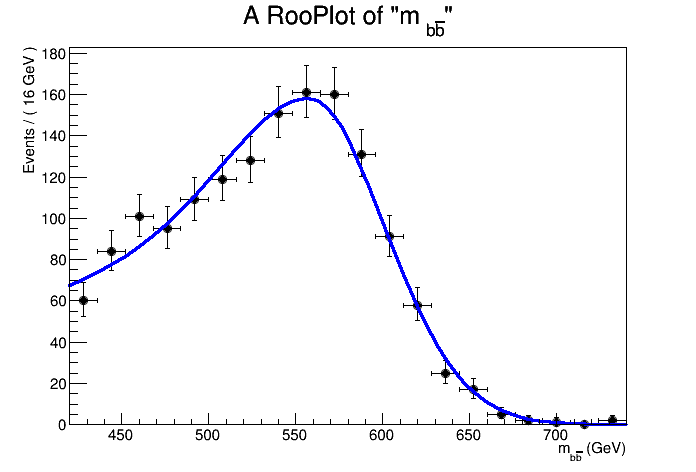
\includegraphics[width=\textwidth]{FitResults/images/fitMC_bAbb600_4.png}\end{subfigure}
  \begin{subfigure}[$m_{A}=650$ GeV]{0.4\textwidth}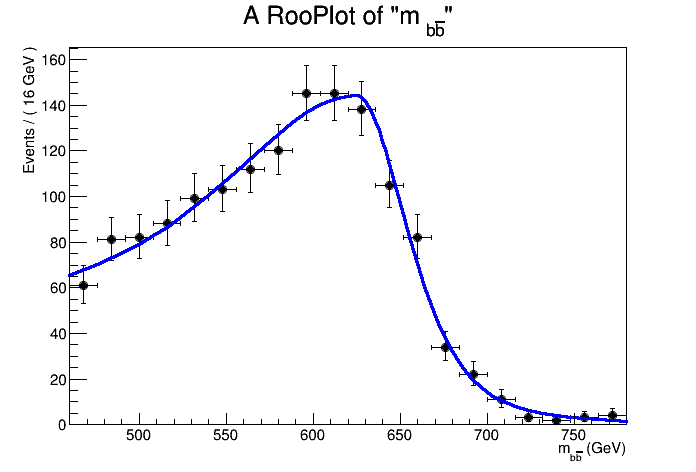
\includegraphics[width=\textwidth]{FitResults/images/fitMC_bAbb650_4.png}\end{subfigure}
  \begin{subfigure}[$m_{A}=700$ GeV]{0.4\textwidth}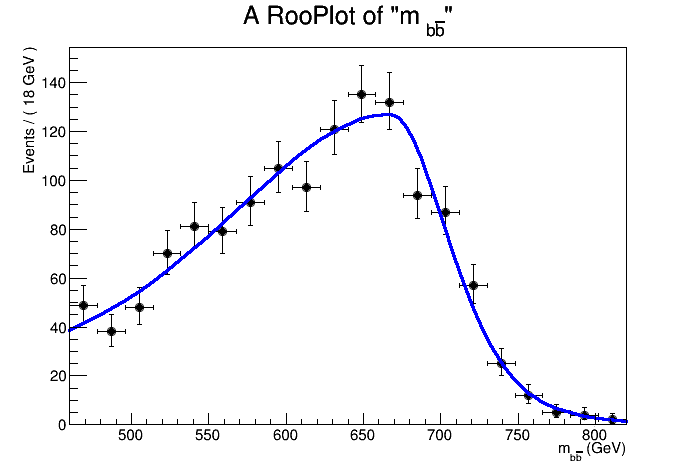
\includegraphics[width=\textwidth]{FitResults/images/fitMC_bAbb700_4.png}\end{subfigure}
  \begin{subfigure}[$m_{A}=800$ GeV]{0.4\textwidth}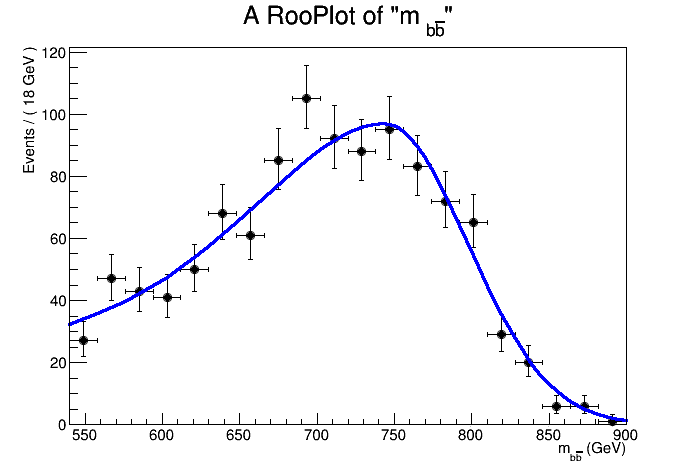
\includegraphics[width=\textwidth]{FitResults/images/fitMC_bAbb800_4.png}\end{subfigure}
  \caption{Signal MC distributions and Cruijff PDFs for $m_{bb}$ in the {\it bbloose} category, for events with 3 jets, for different $H/A$ masses. \label{fig:signalPDFs_3j_bbloose}}
    \end{center}
\end{figure}


\begin{figure}[phtb!]
  \begin{center}
  \begin{subfigure}[$m_{A}=400$ GeV]{0.4\textwidth}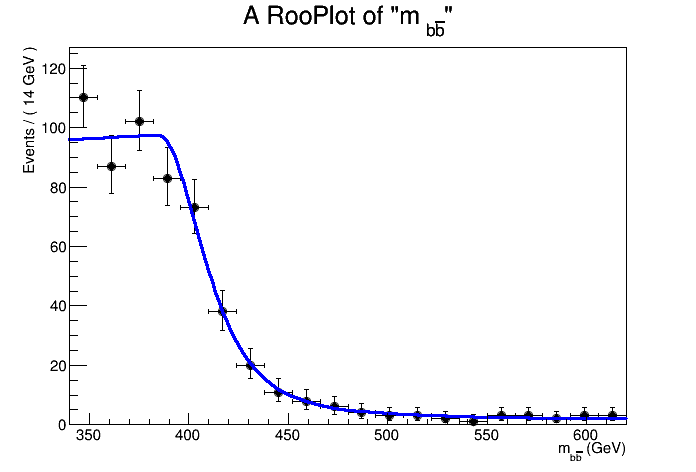
\includegraphics[width=\textwidth]{FitResults/images/fitMC_bAbb400_5.png}\end{subfigure}
  \begin{subfigure}[$m_{A}=450$ GeV]{0.4\textwidth}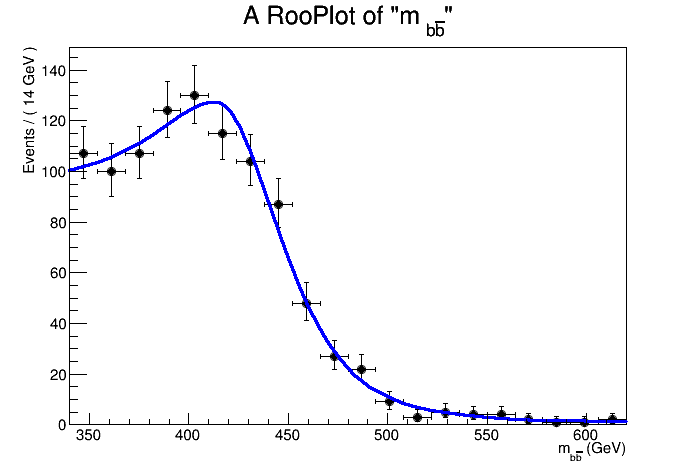
\includegraphics[width=\textwidth]{FitResults/images/fitMC_bAbb450_5.png}\end{subfigure}
  \begin{subfigure}[$m_{A}=500$ GeV]{0.4\textwidth}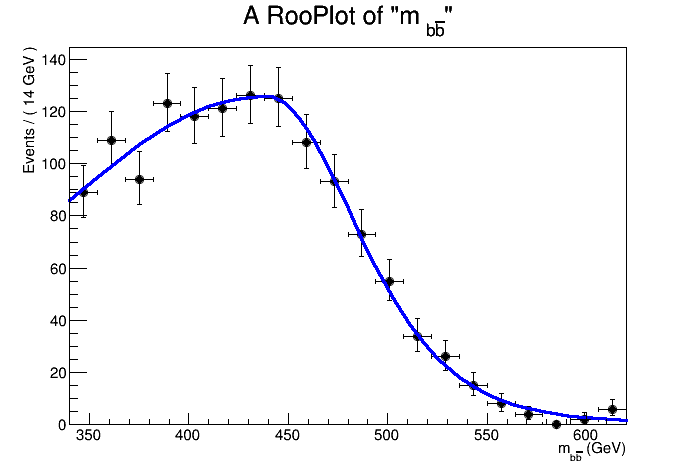
\includegraphics[width=\textwidth]{FitResults/images/fitMC_bAbb500_5.png}\end{subfigure}
  \begin{subfigure}[$m_{A}=550$ GeV]{0.4\textwidth}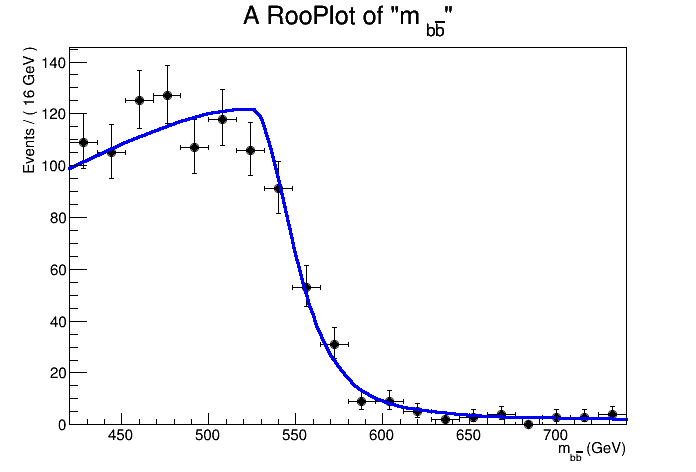
\includegraphics[width=\textwidth]{FitResults/images/fitMC_bAbb550_5.png}\end{subfigure}
  \begin{subfigure}[$m_{A}=600$ GeV]{0.4\textwidth}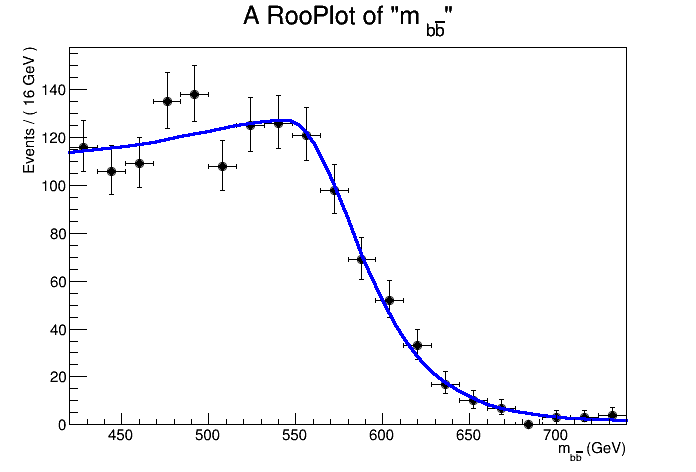
\includegraphics[width=\textwidth]{FitResults/images/fitMC_bAbb600_5.png}\end{subfigure}
  \begin{subfigure}[$m_{A}=650$ GeV]{0.4\textwidth}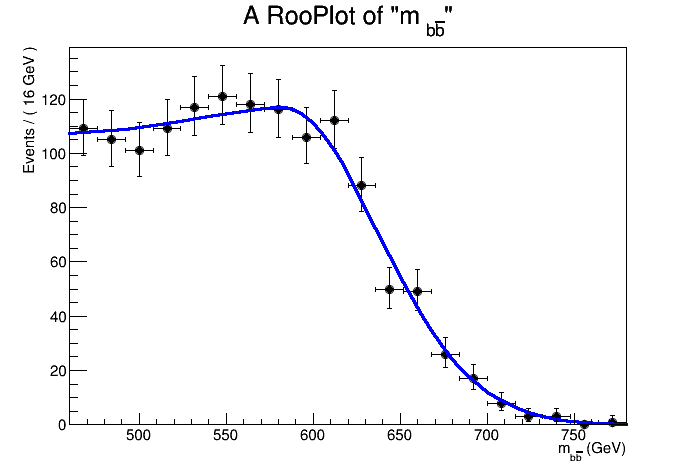
\includegraphics[width=\textwidth]{FitResults/images/fitMC_bAbb650_5.png}\end{subfigure}
  \begin{subfigure}[$m_{A}=700$ GeV]{0.4\textwidth}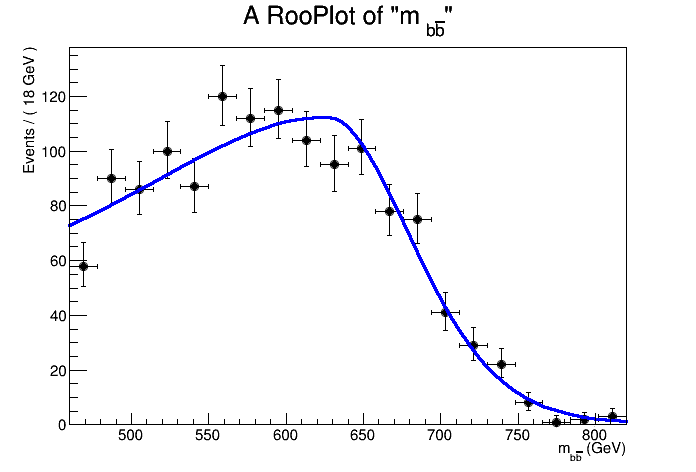
\includegraphics[width=\textwidth]{FitResults/images/fitMC_bAbb700_5.png}\end{subfigure}
  \begin{subfigure}[$m_{A}=800$ GeV]{0.4\textwidth}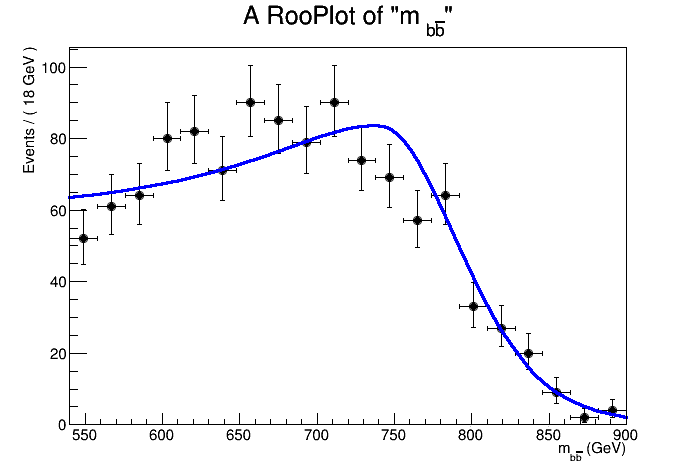
\includegraphics[width=\textwidth]{FitResults/images/fitMC_bAbb800_5.png}\end{subfigure}
  \caption{Signal MC distributions and Cruijff PDFs for $m_{bb}$ in the {\it bbloose} category, for events with 3 jets, for different $H/A$ masses. \label{fig:signalPDFs_4j_bbloose}}
    \end{center}
\end{figure}


\begin{figure}[phtb!]
  \begin{center}
  \begin{subfigure}[$m_{A}=400$ GeV]{0.4\textwidth}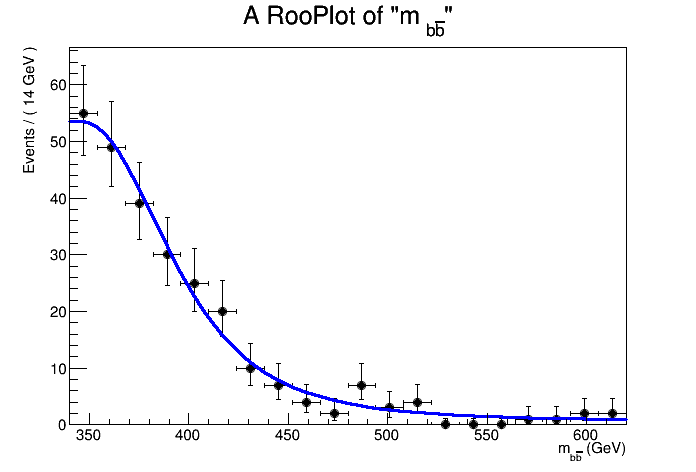
\includegraphics[width=\textwidth]{FitResults/images/fitMC_bAbb400_6.png}\end{subfigure}
  \begin{subfigure}[$m_{A}=450$ GeV]{0.4\textwidth}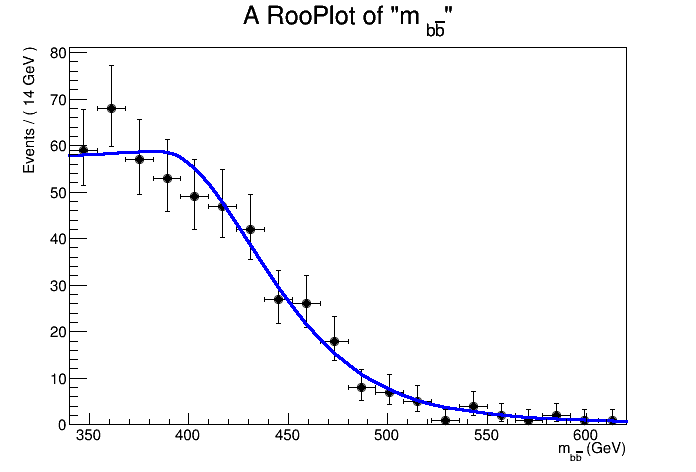
\includegraphics[width=\textwidth]{FitResults/images/fitMC_bAbb450_6.png}\end{subfigure}
  \begin{subfigure}[$m_{A}=500$ GeV]{0.4\textwidth}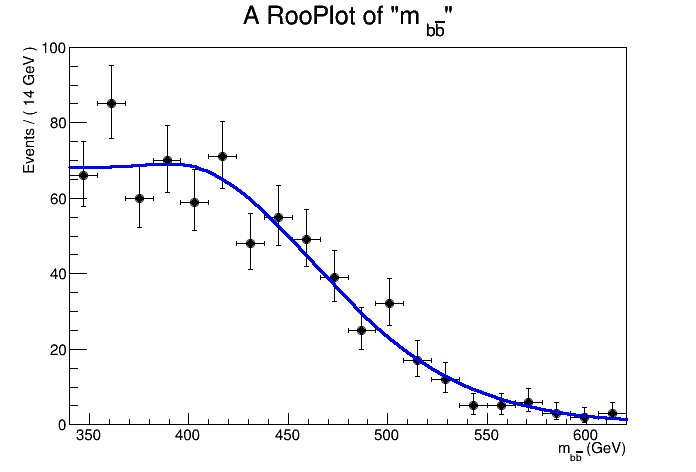
\includegraphics[width=\textwidth]{FitResults/images/fitMC_bAbb500_6.png}\end{subfigure}
  \begin{subfigure}[$m_{A}=550$ GeV]{0.4\textwidth}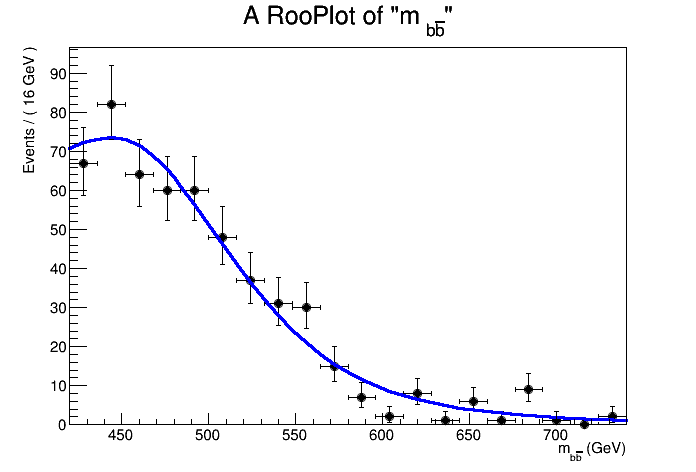
\includegraphics[width=\textwidth]{FitResults/images/fitMC_bAbb550_6.png}\end{subfigure}
  \begin{subfigure}[$m_{A}=600$ GeV]{0.4\textwidth}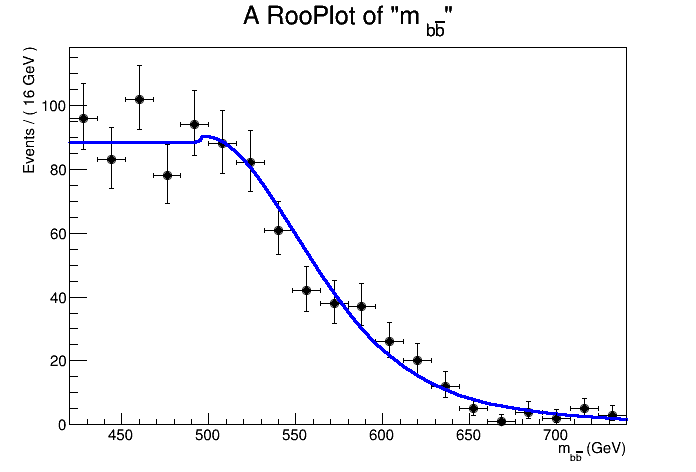
\includegraphics[width=\textwidth]{FitResults/images/fitMC_bAbb600_6.png}\end{subfigure}
  \begin{subfigure}[$m_{A}=650$ GeV]{0.4\textwidth}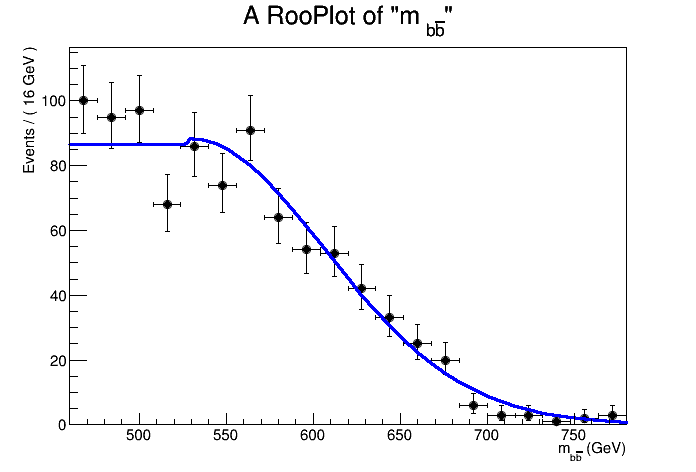
\includegraphics[width=\textwidth]{FitResults/images/fitMC_bAbb650_6.png}\end{subfigure}
  \begin{subfigure}[$m_{A}=700$ GeV]{0.4\textwidth}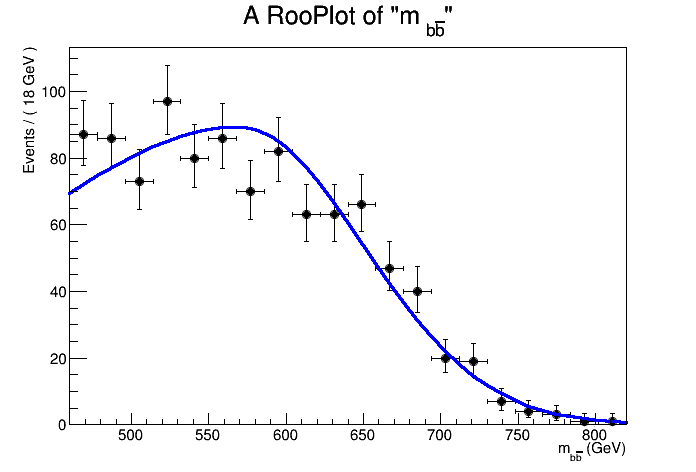
\includegraphics[width=\textwidth]{FitResults/images/fitMC_bAbb700_6.png}\end{subfigure}
  \begin{subfigure}[$m_{A}=800$ GeV]{0.4\textwidth}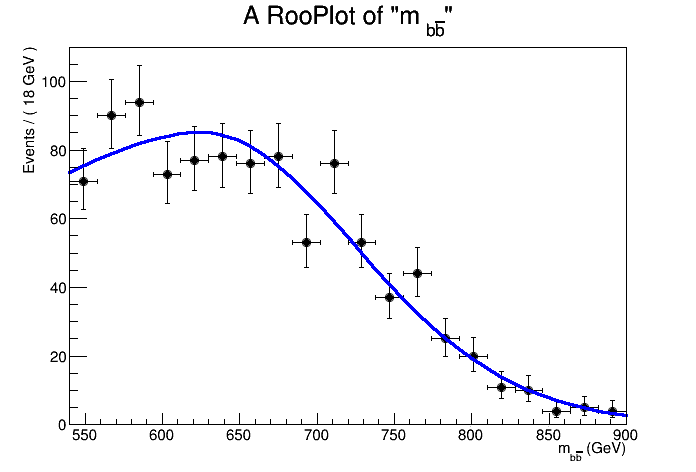
\includegraphics[width=\textwidth]{FitResults/images/fitMC_bAbb800_6.png}\end{subfigure}
  \caption{Signal MC distributions and Cruijff PDFs for $m_{bb}$ in the {\it bbloose} category, for events with 5 or more jets, for different $H/A$ masses. \label{fig:signalPDFs_5j_bbloose}}
    \end{center}
\end{figure}



\section{Limit Extraction}
Once the signal and background have been fit, the CL$_s$ method is used to 
determine the $\sigma\times BR$ that can be excluded at the 95\% confidence
level \cite{CLS1}, \cite{CLS2}, \cite{CLS3}.  The CL$_s$ method is a
frequentist limit-setting procedure that is designed to give upper limits that
are greater than the true value of $\sigma\times BR$ with a probability of at
least 95\%.

Once the signal and background PDF shapes are determined in the fit,
the limit setting procedure proceeds as follows.  The fits are used to generate
an ensemble of toy MC datasets
that are combined into a single representative dataset, called the ``Asimov
The limit-setting procedure 
dataset'' for that distribution.  Then 
In order to obtain the nominal fit result in terms of $\mu$ and $\sigma_{\mu}$
the likelihood function is maximized with respect to all parameters.
This is referred to as the maximized log-likelihood value MLL.
The test statistic $q_\mu$ is then constructed according to
the profile likelihood:
\begin{equation}
q_\mu = 2 \mathrm{ln} (\mathcal{L} (\mu,
\hat{\hat{\theta_\mu}})/\mathcal{L} (\hat{\mu}, \hat{\theta})), 
\end{equation}
where
$\hat{\mu}$ and $\hat{\theta}$ are the parameters that maximize the
likelihood (with the constraint $0 \leq \hat{\mu} \leq \mu$), and
$\hat{\hat{\theta}}_\mu$ are the nuisance parameter values that maximize the
likelihood for a given $\mu$. This test statistic is used to measure
the compatibility of the background only model with the observed
data. 

Expected exlusion limits following this procedure are shown in Fig.~\ref{fig:limitSensitivity} and Table~\ref{tab:limitSensitivity}. These are obtained under the assumption that
 a good estimate of the background parameters is given by the fit values reported in Table~\ref{tab:bkgFit}.

\textbf{table of parameters returned by fit}

\textbf{table of CLs limits by mass point}

\textbf{brazil plot}
